%% -*- coding:utf-8 -*- 
\documentclass[14pt,a4paper]{article} 
\usepackage[utf8]{inputenc}
\usepackage[english]{babel}
\usepackage{minted}
\usepackage{longtable}
\usepackage{hyperref}
\hypersetup{
  pdftex,
  allcolors=blue,
  bookmarksnumbered=true,     
  bookmarksopen=true,         
  bookmarksopenlevel=1,       
  colorlinks=true,            
  pdfstartview=Fit,           
  pdfpagemode=UseOutlines,  
  pdfpagelayout=TwoPageRight,
  pdftitle={Docker tutorial},
  pdfsubject={Docker},
  pdfauthor={Ivan Murashkо},
  pdfkeywords={Docker, tutorial, thrift, php, C++}
}
\usepackage{tikz}
\usetikzlibrary{positioning} 
\title{Docker tutorial}
\author{Ivan Murashko}
\date{}
\begin{document}

\maketitle
\tableofcontents

\section*{Introduction}
There are several examples of docker usage. They are collected in one
place mainly for future references.

The source code for examples can be found in the article git
repository \cite{github:articles_ivanmurashko} in the folder 
\textbf{dockertutorial/src}.

\section{Base commands}

\subsection{Simple program run}
You can run a command (\textbf{uname -a}) with 
\begin{minted}{shell}
$ docker run ubuntu uname -a
\end{minted}
The container \textbf{ubuntu:latest} will be used in the case. 

The command execution status can be viewed with
\begin{verbatim}
$ docker ps -a 
CONTAINER ID   IMAGE   COMMAND     CREATED         ...
b5e8d82cce29   ubuntu  "uname -a"  5 seconds ago  ...
\end{verbatim}
If you run the docker with \textbf{--rm} flag then the status info
will not be stored.


\subsection{Interactive session}
You can run an interactive shell with
\begin{minted}{shell}
$ docker run -it ubuntu /bin/bash
\end{minted}
where \textbf{-it} means \textbf{--interactive --tty}, 
\textbf{ubuntu} the latest ubuntu image and \textbf{/bin/bash} - the
command to be start 

\subsection{Docker as a daemon}
First of all run the docker in interactive mode and as daemon
\begin{minted}{shell}
$ docker run -itd ubuntu
\end{minted}
possible output
\begin{verbatim}
649dae02de59ea3eb065a40b1248b2d322986e563ab12af3126fa4bb4710008a
\end{verbatim}
Check the docker run in daemon mode with
\begin{minted}{shell}
$ docker ps
\end{minted}
output:
\begin{verbatim}
$ docker ps 
CONTAINER ID        IMAGE               COMMAND     ...
649dae02de59        ubuntu              "/bin/bash" ...
\end{verbatim}
Execute \textbf{ls /var} command in the run docker
\begin{verbatim}
$ docker exec -it 649dae02de59 ls /var
backups  cache  lib  local  lock  log  mail  opt  run  spool  tmp
\end{verbatim}
Stop it with
\begin{verbatim}
$ docker stop 649dae02de59
649dae02de59
\end{verbatim}
Check the result
\begin{verbatim}
$ docker ps
CONTAINER ID        IMAGE               COMMAND   ...
\end{verbatim}

\subsection{Network daemon}
You can run a nginx web server with the following command
\begin{verbatim}
$ docker run -p 8080:80 -d nginx
\end{verbatim}
This will map docker container port 80 to the host port 8080 or in
other words make the nginx server available on the host machine via port
8080:
\begin{verbatim}
$ telnet localhost 8080
Trying 127.0.0.1...
Connected to localhost.
Escape character is '^]'.
HEAD / HTTP/1.0

HTTP/1.1 200 OK
Server: nginx/1.17.4
Date: Sat, 28 Sep 2019 18:44:45 GMT
Content-Type: text/html
Content-Length: 612
Last-Modified: Tue, 24 Sep 2019 14:49:10 GMT
Connection: close
ETag: "5d8a2ce6-264"
Accept-Ranges: bytes

Connection closed by foreign host.
\end{verbatim}

\subsection{Stop all}
You can stop all containers with
\begin{verbatim}
$ docker container stop $(docker container ls -aq)
\end{verbatim}

\subsection{Cleanup}
The following command will remove everything
\begin{verbatim}
$ docker system prune -a
WARNING! This will remove:
        - all stopped containers
        - all networks not used by at least one container
        - all images without at least one container associated to them
        - all build cache
Are you sure you want to continue? [y/N] y
Deleted Containers:
b5e8d82cce2942a24c709b630ff4e0dd705b89d78f2777065446ce97cf152cab
...
Total reclaimed space: 6.113GB
\end{verbatim}

\section{Creating docker images}

\subsection{Build}
In the example we will create a docker image that will help us to
compile and run code that uses thrift protocol \cite{apache:thrift}.
The necessary libs for us are C++ and PHP. 

The Dockerfile can be found in the article git
repository \cite{github:articles_ivanmurashko} in the folder 
\textbf{dockertutorial/src/thrift}.
\inputminted{shell}{./src/thrift/Dockerfile}
You can compile it with 
\begin{verbatim}
$ cd src/thrift/
$ docker build -t thriftbuilder .
...
Successfully tagged thriftbuilder:latest
$
\end{verbatim}
You can look at the image with 
\begin{verbatim}
$ docker images
REPOSITORY          TAG                 IMAGE ID            CREATED              SIZE
thriftbuilder       latest              be1ccc48fb53        About a
minute ago
\end{verbatim}
You can test the result with
\begin{verbatim}
$ docker run --rm thriftbuilder  thrift --version
Thrift version 0.12.0
\end{verbatim}
The \textbf{--rm} option is used to be sure that the stopped container
was removed.  

\subsection{Cleanup}
To remove the image you can use
\begin{verbatim}
$ docker image rm thriftbuilder
\end{verbatim}
If you got an error during the removal:
\begin{verbatim}
Error response from daemon: conflict: unable to remove repository
reference "thriftbuilder" (must force) - container dc0836d6f65f is
using its referenced image be1ccc48fb53
\end{verbatim}
then try to remove the stopped container before
\begin{verbatim}
$ docker container rm dc0836d6f65f
\end{verbatim}
TBD

\section{Apps in docker}
I am going to create a small application that consists of 2 parts. The
first one is front-end written in php that communicates with a back-end server
written in C++. The communication is done via thrift protocol
\cite{apache:thrift}. The front-end server as well as back-end server
are run in different container and all communication is done via the
network. 

\begin{figure}
  \centering
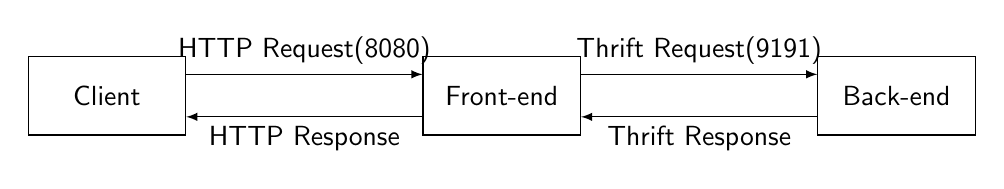
\begin{tikzpicture}[block/.style={draw,minimum width=2cm,minimum height=1cm}, font=\sffamily] 
\node[block](C) {Client}; 
\node[block,right=3cm of C](F) {Front-end}; 
\node[block,right=3cm of F](B) {Back-end}; 
\draw[-latex] (C.15) -- (F.165)
node[midway,above]{HTTP Request(8080)}; 
\draw[-latex] (F.195) -- (C.-15) node[midway,below]{HTTP Response}; 
\draw[-latex] (F.15) -- (B.165)
node[midway,above]{Thrift Request(9191)}; 
\draw[-latex] (B.195) -- (F.-15) node[midway,below]{Thrift Response}; 
\end{tikzpicture} 
  \caption{Applications}
  \label{fig:apps}
\end{figure}
The client (see \ref{fig:apps}) is run on a host and communicates
with front-end run in a docker container via HTTP protocol, port 8080
is used. The front-end communicates with a back-end application that
is run on another docker container. The communication is done via 9191
port. 

\subsection{Build and run back-end (C++) application}
We are going to create a separate docker image for C++ application.
The image Dockerfile can be found in the article git
repository \cite{github:articles_ivanmurashko} in the folder 
\textbf{dockertutorial/src/cpp}.
\inputminted{shell}{./src/cpp/Dockerfile}
As you can see it is based on the thriftbuilder image created before. 

The daemon can be built with the following command run from
\textbf{./src} folder:
\begin{verbatim}
$ docker build -t cppapp -f cpp/Dockerfile .
\end{verbatim}
It also builds the application inside the docker. It can be run as
follows
\begin{verbatim}
$ docker run --rm -p 9191:9191 -d cppapp
\end{verbatim}

The application code can be found in \textbf{dockertutorial/src/cpp} folder:
\inputminted{c++}{./src/cpp/main.cpp}


\subsection{Build and run front-end (php) application}
We are going to create a separate image for front-end application. The
image will be based on the thriftbuilder image created before.
It will install and setup apache web server to work with php content.
The setup instruction was taken from \cite{apache:php}.
The image Dockerfile can be found in the article git
repository \cite{github:articles_ivanmurashko} in the folder 
\textbf{dockertutorial/src/php}.
\inputminted{shell}{./src/php/Dockerfile}
The daemon can be built with the following command run from
\textbf{./src} folder:
\begin{verbatim}
$ docker build -t phpapp -f php/Dockerfile .
\end{verbatim}
It also builds the application inside the docker. It can be run as
follows
\begin{verbatim}
$ docker run --rm -p 8080:80 -d phpapp
\end{verbatim}

The application code can be found in \textbf{dockertutorial/src/php} folder:
\inputminted{php}{./src/php/index.php}

\subsection{Test}
First of all start the required containers if them have not been
started before
\begin{verbatim}
$ docker run --rm -p 9191:9191 -d cppapp
b6ae2f7687b56d9d68028a38aa5f3357cdf096cfa0ead83768e17b4d270edf23
$ docker run --rm -p 8080:80 -d phpapp
d8d3ea9415ac614df623c30abf70c48030f03c81ae922e541085cfb082d4e4c4
\end{verbatim}
The font-end can be tested via telnet as follow
\begin{verbatim}
$ telnet localhost 8080
Trying 127.0.0.1...
Connected to localhost.
Escape character is '^]'.
GET / HTTP/1.0

HTTP/1.1 200 OK
Date: Thu, 03 Oct 2019 14:33:00 GMT
Server: Apache/2.4.29 (Ubuntu)
Content-Length: 54
Connection: close
Content-Type: text/html; charset=UTF-8

Current time from back-end: Thu Oct  3 14:33:00 2019

Connection closed by foreign host.
\end{verbatim}

\bibliographystyle{unsrt}  
\bibliography{dockertutorial}     


\end{document}
